\documentclass[a4paper]{article} 
\usepackage{graphicx} 
\usepackage[ngerman]{babel} 
\usepackage[ansinew]{inputenc} 
\usepackage[T1]{fontenc} 
\usepackage{tgpagella} 
\usepackage{geometry} 
\usepackage{color} 
\usepackage{microtype} 
\usepackage{minted}
\usepackage{caption}
\usepackage[headsepline,footsepline]{scrpage2}
\usepackage{textcomp}
\usepackage{pdfpages}
\usepackage{mdframed}



\makeatletter
\renewcommand\minted@pygmentize[2][\jobname.pyg]{
  \def\minted@cmd{pygmentize -l #2 -f latex -F tokenmerge
    \minted@opt{gobble} \minted@opt{texcl} \minted@opt{mathescape}
    \minted@opt{startinline} \minted@opt{funcnamehighlighting}
    \minted@opt{linenos} -P "verboptions=\minted@opt{extra}"
    -O encoding=UTF-8,outencoding=iso-8859-1 -o \jobname.out.pyg #1}
  \immediate\write18{\minted@cmd}
  % For debugging, uncomment:
  %\immediate\typeout{\minted@cmd}
  \ifthenelse{\equal{\minted@opt@bgcolor}{}}
   {}
   {\begin{minted@colorbg}{\minted@opt@bgcolor}}
  \input{\jobname.out.pyg}
  \ifthenelse{\equal{\minted@opt@bgcolor}{}}
   {}
   {\end{minted@colorbg}}
  \DeleteFile{\jobname.out.pyg}}
\makeatother


\title{Dokumentation - 6 Übung}
\author{Roman Lumetsberger}
\date{\today}

\newmintedfile[ccode]{cpp}{
               linenos,
               numbersep=5pt,
               frame=lines,
               framesep=2mm
}

\newmintedfile[javacode]{java}{
               linenos,
               numbersep=5pt,
               frame=lines,
               tabsize=2,
               framesep=2mm,
}
\newmintedfile[csscode]{css}{
               linenos,
               numbersep=5pt,
               frame=lines,
               tabsize=2,
               framesep=2mm,
}
\newmintedfile[sqlcode]{sql}{
               linenos,
               numbersep=5pt,
               frame=lines,
               tabsize=2,
               framesep=2mm,
}
\captionsetup{
  font=footnotesize,
  justification=raggedright,
  singlelinecheck=false
}


\newcommand{\srcDir}{../Beispiel/src/at/lumetsnet/caas/}
\newcommand{\testDir}{../Beispiel/test/at/lumetsnet/caas/test/}

\definecolor{lineColor}{RGB}{151,0,0}
\pagestyle{scrheadings}
\clearscrheadfoot
\begin{document}
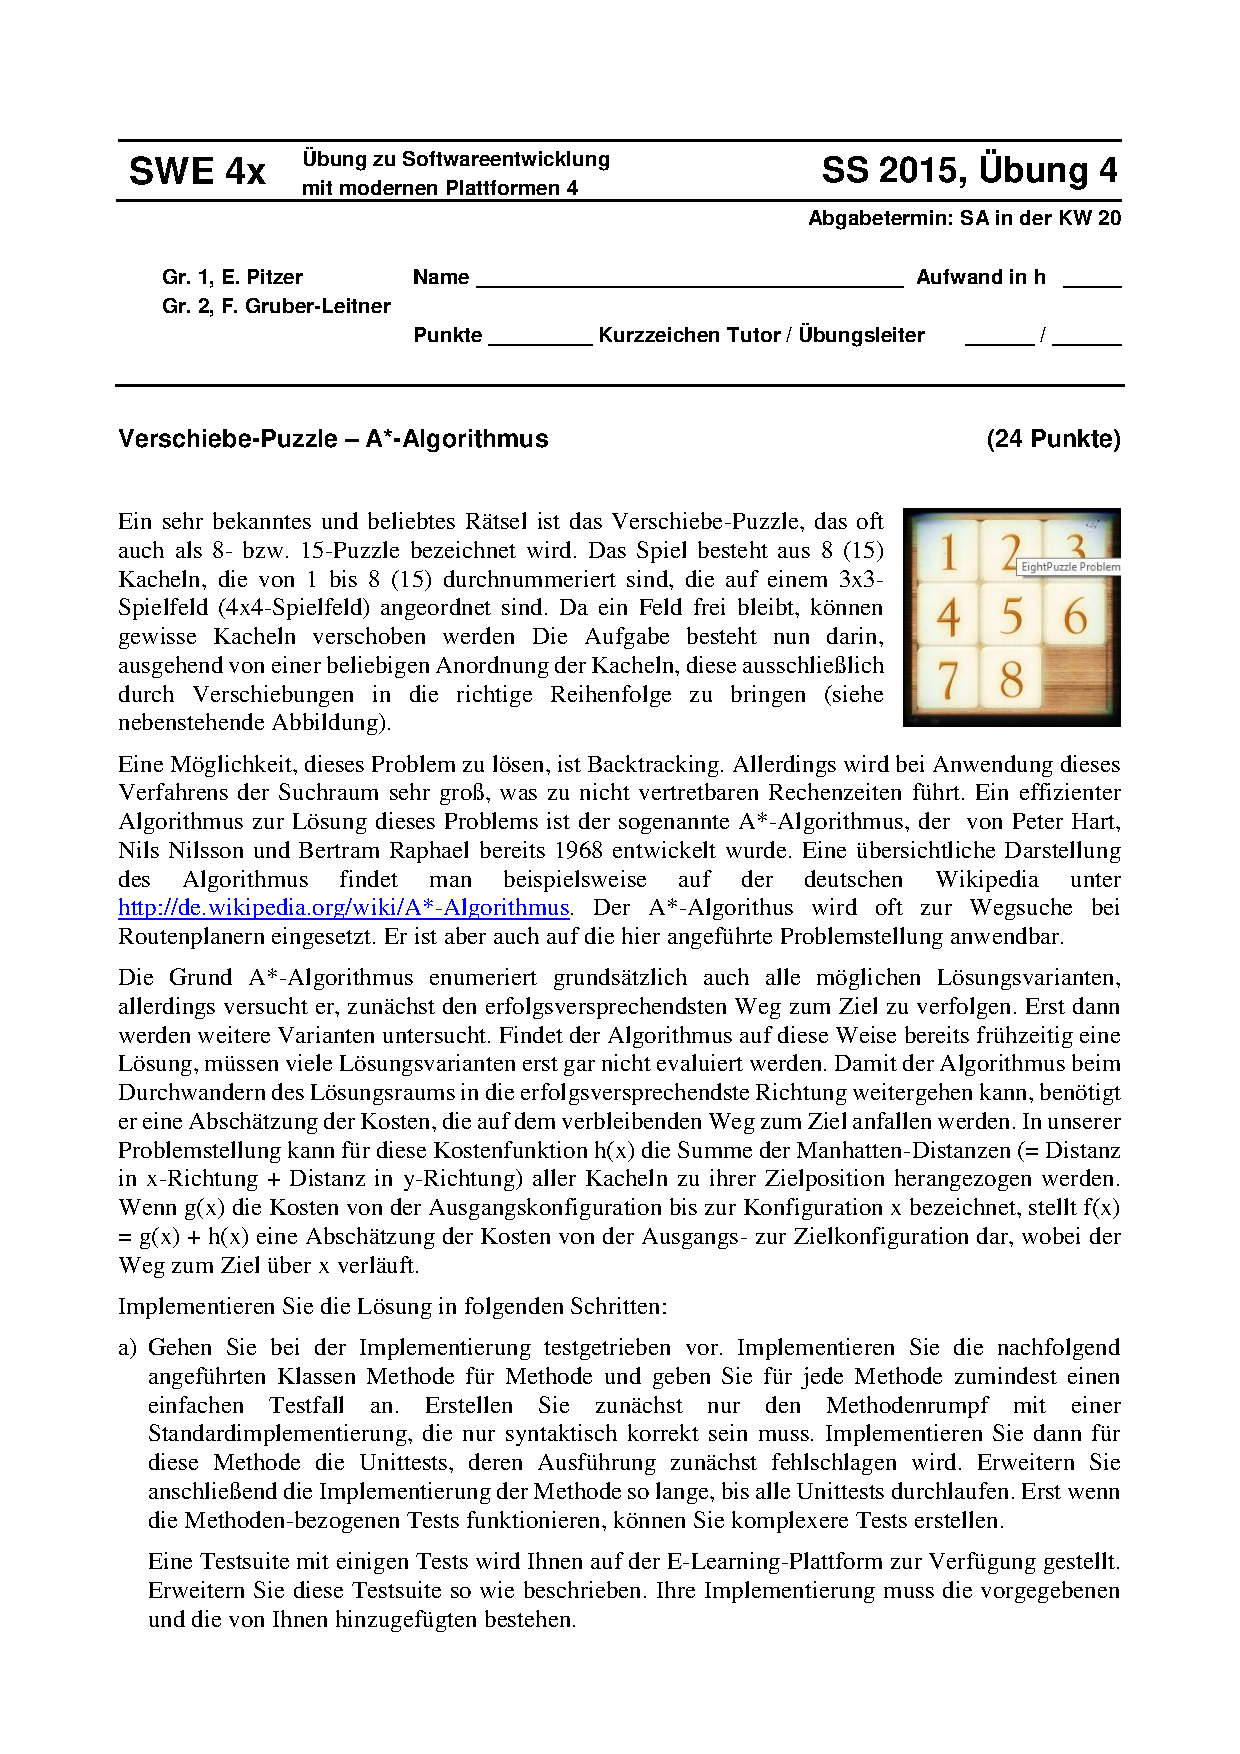
\includepdf[pages=-]{angabe.pdf}

\ihead{SWO3 SS 2015 - �bung 04}
\ifoot{Roman Lumetsberger}
\cfoot{1310307026}
\ofoot{Seite \pagemark}

\section{Verschiebe-Puzzle � A*-Algorithmus }
\subsection{L�sungsidee}
Als ersten Schritt der L�sung werden die, in der Angabe erw�hnten, Klassen implementiert und die Testf�lle erweitert.
Dabei ist die Implementierung der meisten Methoden trivial. \newline
Im folgenden werden nur mehr jede L�sungsideen angef�hrt, die mehr �berlegungen erfordern.

\subsubsection{Board}
Die Klasse \textit{Board} verwendet als Datenspeicher eine \textit{ArrayList}, wobei hier der Zeilen und Spaltenindex auf den Index in der \textit{ArrayList} abgebildet werden muss.\newline

\subsubsection{SearchNode - calcManhattanDistance}
Die Manhattan Distance wird in der Klasse \textit{SearchNode} berechnet und wird f�r den A* Algorithmus ben�tigt.\newline
Dabei wird das gesamte Board durchlaufen und f�r jedes Element die Abweichung zur Zielkonfiguration berechnet.\newline
Die Zielposition kann folgenderma�en berechnet werden:
\begin{itemize}
	\item Zeile: Nummer / Gr��e des Boards
	\item Spalte: Nummer \% Gr��e des Boards
\end{itemize} 
Die Manhattan Distance errechnet sich dann aus den Summen der Abweichungen der einzelnen Positionen.

\subsubsection{SearchNode - toMoves}
Um die Liste der Z�ge vom Start bis zur aktuellen Konfiguration zu berechnen, muss die verkette Liste aufgel�st werden.\newline
Das Ergebnis muss dann noch umgedreht werden, da wir ja die Z�ge vom Start bis zum Ziel ben�tigen.

\subsubsection{SlidingPuzzle - solve}
Um das Verschiebe-Puzzle zu l�sen wird, wie in der Angabe erw�hnt, der A* Algorithmus angewendet. \newline
Dieser ben�tigt eine \textbf{openQueue} und ein \textbf{closedSet}.
\begin{itemize}
	\item openQueue: enth�lt die noch zu pr�fenden Pfade sortiert nach ihren Kosten zum Ziel. (Darum kann hier eine \textit{PriorityQueue} verwendet werden.)
	\item closedSet: enth�lt die bereits gepr�ften Pfade.
\end{itemize}

\textbf{Ablauf:}
\begin{itemize}
	\item Zu Begin wird die Startkonfiguration in die \textbf{openQueue} eingef�gt.
	\item In einer Schleife wird dann das oberste Element der Queue herausgenommen.
	\item Ist das Element die Zielkonfiguration, wurde eine L�sung gefunden.
	\item Wenn nicht, wird das Element in das \textbf{closedSet} eingef�gt.
	\item Dann werden alle Nachfolger berechnet. (g�ltige Verschiebeoperationen anwenden)
	\item Jeder Nachfolger wird dann in die \textbf{openQueue} eingef�gt, wenn er noch nicht betrachtet wurde oder seine Kosten geringer sind.
\end{itemize}


\pagebreak
\subsection{Sourcecode}

\textbf{Board.java}
\javacode{\srcDir/Board.java}
\textbf{Move.java}
\javacode{\srcDir/Move.java}
\textbf{SearchNode.java}
\javacode{\srcDir/SearchNode.java}	
\textbf{SlidingPuzzle.java}
\javacode{\srcDir/SlidingPuzzle.java}
\textbf{BoardException.java}
\javacode{\srcDir/exceptions/BoardException.java}
\textbf{IllegalMoveException.java}
\javacode{\srcDir/exceptions/IllegalMoveException.java}
\textbf{InvalidBoardIndexException.java}
\javacode{\srcDir/exceptions/InvalidBoardIndexException.java}
\textbf{InvalidTileNumberException.java}
\javacode{\srcDir/exceptions/InvalidTileNumberException.java}
\textbf{NoSolutionException.java}
\javacode{\srcDir/exceptions/NoSolutionException.java}
\textbf{AbstractTest.java}
\javacode{\srcDir/tests/AbstractTest.java}
\textbf{BoardTest.java}
\javacode{\srcDir/tests/BoardTest.java}
\textbf{SearchNodeTest.java}
\javacode{\srcDir/tests/SearchNodeTest.java}
\textbf{SlidingPuzzleSolverTest.java}
\javacode{\srcDir/tests/SlidingPuzzleSolverTest.java}



\subsection{Testf�lle}
\begin{center}

\end{center}



\end{document}